
%(BEGIN_QUESTION)
% Copyright 2006, Tony R. Kuphaldt, released under the Creative Commons Attribution License (v 1.0)
% This means you may do almost anything with this work of mine, so long as you give me proper credit

A liquid storage vessel holding a very corrosive liquid has its level measured by a {\it bubbler} system, whereby a transmitter measures the backpressure of air inside a ``dip tube'' inserted into the vessel:

$$\includegraphics[width=15.5cm]{i00249x01.eps}$$

Explain how this level measurement system works, and how it protects the DP cell from the corrosive effects of the process liquid.

\vskip 10pt

Also, complete a calibration table for the differential pressure transmitter in this level measurement scenario, with a calibration tolerance of $\pm$ 0.5\%.  Assume that the lower range-value of the process (0\% level) is exactly the same height as the bottom of the dip tube:

% No blank lines allowed between lines of an \halign structure!
% I use comments (%) instead, so that TeX doesn't choke.

$$\vbox{\offinterlineskip
\halign{\strut
\vrule \quad\hfil # \ \hfil & 
\vrule \quad\hfil # \ \hfil & 
\vrule \quad\hfil # \ \hfil & 
\vrule \quad\hfil # \ \hfil & 
\vrule \quad\hfil # \ \hfil & 
\vrule \quad\hfil # \ \hfil \vrule \cr
\noalign{\hrule}
%
% First row
Process & Percent of & $\Delta$ pressure & Output signal & Output signal & Output signal \cr
%
% Another row
level (ft) & span (\%) & sensed ("W.C) & ideal (mA) & min. (mA) & max. (mA) \cr
%
\noalign{\hrule}
%
% Another row
  & 0 &  &  &  &  \cr
%
\noalign{\hrule}
%
% Another row
  & 10 &  &  &  &  \cr
%
\noalign{\hrule}
%
% Another row
  & 25 &  &  &  &  \cr
%
\noalign{\hrule}
%
% Another row
  & 50 &  &  &  &  \cr
%
\noalign{\hrule}
%
% Another row
  & 75 &  &  &  &  \cr
%
\noalign{\hrule}
%
% Another row
  & 90 &  &  &  &  \cr
%
\noalign{\hrule}
%
% Another row
  & 100 &  &  &  &  \cr
%
\noalign{\hrule}
} % End of \halign 
}$$ % End of \vbox

\vskip 20pt \vbox{\hrule \hbox{\strut \vrule{} {\bf Suggestions for Socratic discussion} \vrule} \hrule}

\begin{itemize}
\item{} The dip tube (or ``bubbler'') system does indeed isolate the transmitter from the corrosive process liquid, but how can the dip tube itself survive?  And, if the dip tube is able to survive in the corrosive liquid (just like the vessel), why can't we find a DP cell that can handle it directly without the isolation of a dip tube system?
\item{} Demonstrate how to {\it estimate} numerical answers for this problem without using a calculator.
\item{} What is your recommendation for setting the position of the needle valve in this bubble tube system?  Exactly how far open is ``open enough,'' and more importantly for what reason?
\item{} What would happen if the end of the dip tube were to become plugged with debris, blocking all flow?
\item{} What would happen if the needle valve were to become plugged with debris, blocking all flow?
\item{} What would happen if the pressure regulator were to become plugged with debris, blocking all flow?
\item{} Add one or more hand valves to the tubing in this system to provide operators with a simple means of unblocking a plugged dip tube using high-pressure compressed air.
\item{} Given a 100\% full vessel, calculate the amount of pressure that would be registered by a pressure gauge connected to the bottom of the vessel.
\item{} Given a 100\% full vessel, calculate the amount of pressure that would be registered by a pressure gauge connected to the bottom of the dip tube.
\item{} Given a 100\% full vessel, calculate the amount of pressure that would be registered by a pressure gauge connected to the transmitter's ``H'' port.
\item{} Given a 100\% full vessel, calculate the amount of pressure that would be registered by a pressure gauge connected to the downstream side of the needle valve.
\item{} Given a 100\% full vessel, calculate the amount of pressure that would be registered by a pressure gauge connected to the upstream side of the needle valve.
\end{itemize}

\underbar{file i00249}
%(END_QUESTION)





%(BEGIN_ANSWER)

\noindent
{\bf Partial answer:}

% No blank lines allowed between lines of an \halign structure!
% I use comments (%) instead, so that TeX doesn't choke.

$$\vbox{\offinterlineskip
\halign{\strut
\vrule \quad\hfil # \ \hfil & 
\vrule \quad\hfil # \ \hfil & 
\vrule \quad\hfil # \ \hfil & 
\vrule \quad\hfil # \ \hfil & 
\vrule \quad\hfil # \ \hfil & 
\vrule \quad\hfil # \ \hfil \vrule \cr
\noalign{\hrule}
%
% First row
Process & Percent of & $\Delta$ pressure & Output signal & Output signal & Output signal \cr
%
% Another row
level (ft) & span (\%) & sensed ("W.C) & ideal (mA) & min. (mA) & max. (mA) \cr
%
\noalign{\hrule}
%
% Another row
0  & 0 &  &  &  &  \cr
%
\noalign{\hrule}
%
% Another row
  & 10 &  &  &  &  \cr
%
\noalign{\hrule}
%
% Another row
  & 25 & 81.31 & 8 &  &  \cr
%
\noalign{\hrule}
%
% Another row
  & 50 &  &  &  & 12.08 \cr
%
\noalign{\hrule}
%
% Another row
  & 75 &  &  &  &  \cr
%
\noalign{\hrule}
%
% Another row
  & 90 &  &  & 18.32 &  \cr
%
\noalign{\hrule}
%
% Another row
18 & 100 & 325.24 &  &  &  \cr
%
\noalign{\hrule}
} % End of \halign 
}$$ % End of \vbox

%(END_ANSWER)





%(BEGIN_NOTES)

% No blank lines allowed between lines of an \halign structure!
% I use comments (%) instead, so that TeX doesn't choke.

$$\vbox{\offinterlineskip
\halign{\strut
\vrule \quad\hfil # \ \hfil & 
\vrule \quad\hfil # \ \hfil & 
\vrule \quad\hfil # \ \hfil & 
\vrule \quad\hfil # \ \hfil & 
\vrule \quad\hfil # \ \hfil & 
\vrule \quad\hfil # \ \hfil \vrule \cr
\noalign{\hrule}
%
% First row
Process & Percent of & $\Delta$ pressure & Output signal & Output signal & Output signal \cr
%
% Another row
level (ft) & span (\%) & sensed ("W.C) & ideal (mA) & min. (mA) & max. (mA) \cr
%
\noalign{\hrule}
%
% Another row
0 & 0 & 0 & 4 & 3.92 & 4.08 \cr
%
\noalign{\hrule}
%
% Another row
1.8 & 10 & 32.52 & 5.6 & 5.52 & 5.68 \cr
%
\noalign{\hrule}
%
% Another row
4.5 & 25 & 81.31 & 8 & 7.92 & 8.08 \cr
%
\noalign{\hrule}
%
% Another row
9 & 50 & 162.62 & 12 & 11.92 & 12.08 \cr
%
\noalign{\hrule}
%
% Another row
13.5 & 75 & 243.93 & 16 & 15.92 & 16.08 \cr
%
\noalign{\hrule}
%
% Another row
16.2 & 90 & 292.71 & 18.4 & 18.32 & 18.48 \cr
%
\noalign{\hrule}
%
% Another row
18 & 100 & 325.24 & 20 & 19.92 & 20.08 \cr
%
\noalign{\hrule}
} % End of \halign 
}$$ % End of \vbox






\filbreak \vskip 20pt \vbox{\hrule \hbox{\strut \vrule{} {\bf Virtual Troubleshooting} \vrule} \hrule}

\noindent
{\bf Predicting the effect of a given fault:} present each of the following faults to the students, one at a time, having them comment on all the effects each fault would produce.

\begin{itemize}
\item{} 
\item{} 
\item{} 
\end{itemize}


\vskip 10pt


\noindent
{\bf Identifying possible/impossible faults:} present symptoms to the students and then have them determine whether or not a series of suggested faults could account for all the symptoms, explaining {\it why} or {\it why not} for each proposed fault:

\begin{itemize}
\item{} Symptom: {\it }
\item{}  -- {\bf Yes/No}
\item{}  -- {\bf Yes/No}
\item{}  -- {\bf Yes/No}
\end{itemize}


\vskip 10pt


\noindent
{\bf Determining the utility of given diagnostic tests:} present symptoms to the students and then propose the following diagnostic tests one by one.  Students rate the value of each test, determining whether or not it would give useful information (i.e. tell us something we don't already know).  Students determine what different results for each test would indicate about the fault, if anything:

\begin{itemize}
\item{} Symptom: {\it Transmitter registers a falsely high liquid level at a remote indicator}
\item{} Change needle valve position -- {\bf Yes} (checks to see if purge rate is too high)
\item{} Crack tube fitting open at the tee -- {\bf Yes} (checks the transmitter's zero)
\item{} Measure transmitter output current -- {\bf Yes} (checks calibration of indicator)
\item{} Crack tube fitting at entry of needle valve -- {\bf No}
\item{}  -- {\bf Yes/No}
\end{itemize}


\vskip 10pt


\noindent
{\bf Diagnosing a fault based on given symptoms:} imagine the ??? fails ??? in this system (don't reveal the fault to students!).  Present the operator's observation(s) to the students, have them consider possible faults and diagnostic strategies, and then tell them the results of tests they propose based on the following symptoms, until they have properly identified the nature and location of the fault:

\begin{itemize}
\item{} Operator observation: {\it }
\item{} 
\item{} 
\end{itemize}
%INDEX% Calibration: table, level transmitter
%INDEX% Measurement, level: bubble tube (bubbler)
%INDEX% Measurement, level: calibration table
%INDEX% Measurement, level: dip tube
%INDEX% Measurement, level: hydrostatic pressure

%(END_NOTES)


